\documentclass[a4paper,12pt]{report}
\usepackage[utf8]{inputenc}
\usepackage[francais]{babel}
\usepackage{fancyhdr}
\usepackage{graphicx}
\usepackage{tikz}
\usetikzlibrary{calc}
\usepackage{listings}
\usepackage{xcolor}
\definecolor{grey}{rgb}{0.9,0.9,0.9}
\usepackage{titlesec}
\usepackage{verbatim}
\usepackage{listings}
\usepackage{textcomp}
\usepackage{hyperref}
\usepackage{ amssymb }


\frenchbsetup{StandardLists=true}
\newcommand{\marge}{18mm}
\usepackage[left=\marge,right=\marge,top=\marge,bottom=\marge]{geometry}
\pagestyle{fancy}
\setlength{\headheight}{14pt}
\chead{
  \textbf{Binôme :} Douaille Erwan \& Yanis Nait Abdelaziz
  \hspace{2em}
  \textbf{Groupe :} M1 Info TI}
\renewcommand{\headrulewidth}{1pt}
\linespread{1}
\setlength{\columnseprule}{0.2pt}


\begin{document}



\makeatletter
\begin{titlepage}
\centering
\vspace{-10em}
{\LARGE \textbf{\textsc{Rapport de Projet RVI}}}\\
\vspace{3em}

\includegraphics[scale=0.6]{image/thalassa.png}\\
\vspace{3em}
{\LARGE \textsc{Projet Thalassa: simulation de plongée sous-marine}}\\

\vspace{8em}
Par\\
\vspace{1em}
{\LARGE \@author}\\

\vspace{2em}



\begin{tikzpicture}[remember picture,overlay]

\node [below left,xshift=-1cm, yshift=4cm] at (current page.south east){
\includegraphics[scale=0.6]{image/ustl1.png}};

\end{tikzpicture}
\end{titlepage}
\makeatother

\sloppy

\setcounter{page}{1} 
\newpage

\section*{Introduction}
Dans ce TP, nous allons voir comment projeter un point se trouvant dans un espace 3D dans un espace 2D. Cette procédure va se baser sur les coordonnées homogènes de ce point. Pour pouvoir calculer les nouvelles coordonnées d’un point dans l’espace 3D, nous devons calculer les matrices extrinsèque et intrinsèque ainsi que la matrice de projection relative à la caméra. 




\section*{Modèles d'objets 3D et affichage 2D}
Dans cette partie nous avons appris à manipuler les coordonnées homogènes d’un point. On dessine un cube 3D composé de plusieurs points et de segments. Pour représenter ce cube on place plusieurs points 3D (x,y,z) en ajoutant une quatrième coordonnée. Cela nous permet d’obtenir une matrice en cordonnées homogènes, qui nous permettront de faire des transformations sur notre vecteur tout en ayant plusieurs interprétations possibles.

\begin{figure}[!ht]
	\center
	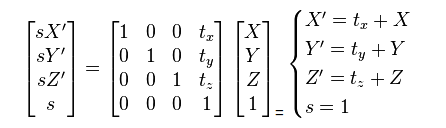
\includegraphics[scale=0.5]{equation.png}
\end{figure}

Avec les matrices extrinsèques nous nous servirons de ces propriétés.
Tout d’abord nous avons dessiné deux cubes et deux grilles avec des dimensions différentes. On peut remarquer que le changement d’échelle garde les rapport de dimensions des cotés ainsi que le parallélisme entre ces derniers.
\begin{center}
\begin{figure}[!ht]
\center
	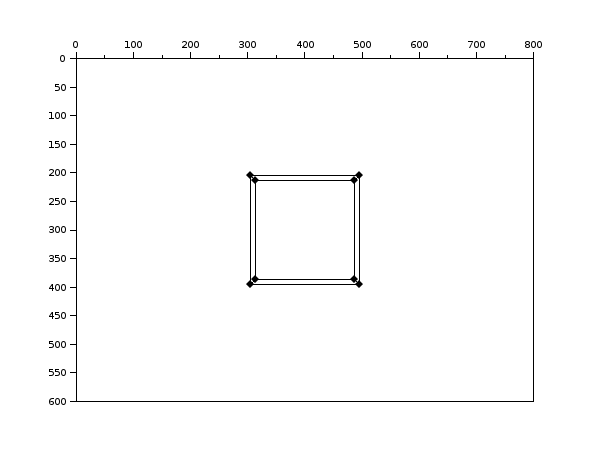
\includegraphics[scale=0.3]{cube00.png}
	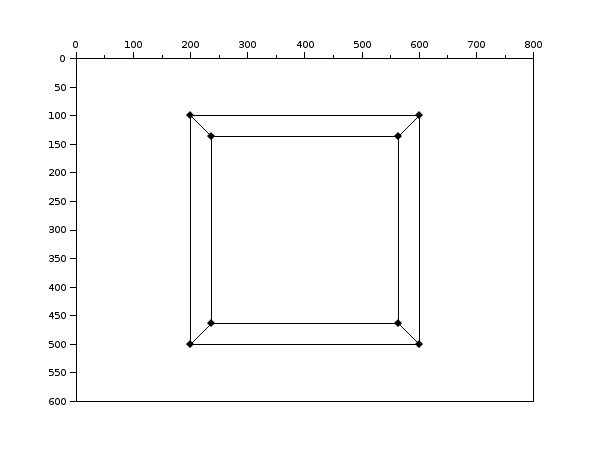
\includegraphics[scale=0.3]{cube_1.png}
\end{figure}
\begin{figure}[!ht]
\center
	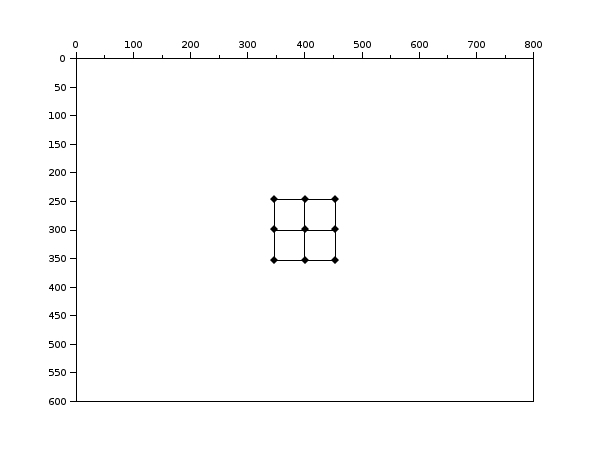
\includegraphics[scale=0.3]{grille_00.png}
	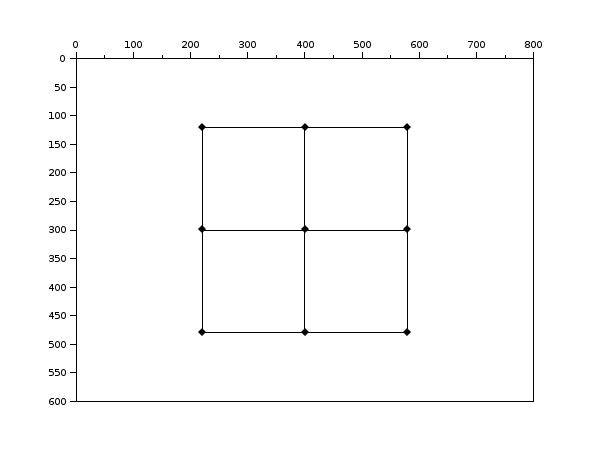
\includegraphics[scale=0.3]{grille_22_1.png}
\end{figure}

\end{center}

Cette premiere etape nous a familiariser avec les outils qui nous sont fournis, la projection, l’encodage des points.

\newpage

\section*{Matrices extrinsèques}
La matrice extrinsèque d’une caméra permet de définir la position et l’orientation de celle-ci par rapport au repère de la scène. En effet celle-ci contient trois paramètres de rotation et trois paramètres de translation.

Pour calculer la matrice extrinsèque positionnant la caméra de centre optique (0, 0, -5 m), axe optique orienté selon z, verticale de la caméra selon y, nous devons juste appliquer une translation selon le vecteur (0,0,5). Ainsi avec ce calcul on obtient la matrice suivante:

\[
   \left (
   \begin{array}{cccc}
      1.0 &   0.0  &  0.0  &  0.0\\
0.0  &  1.0  &  0.0  &  0.0\\
0.0  &  0.0  &  1.0  &  5.0\\
0.0  &  0.0 &   0.0  &  1.0
   \end{array}
   \right )
\]



\begin{figure}[!ht]
\center
	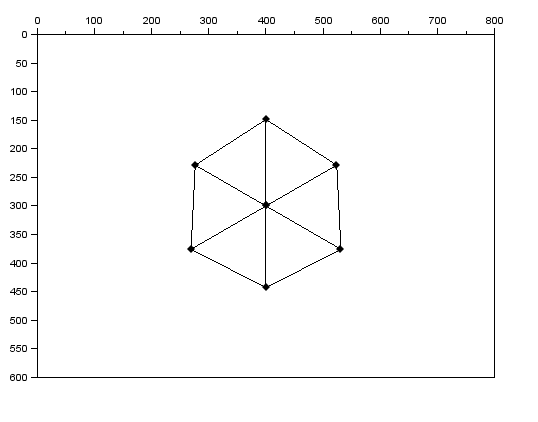
\includegraphics[scale=0.5]{cube_4.png}
	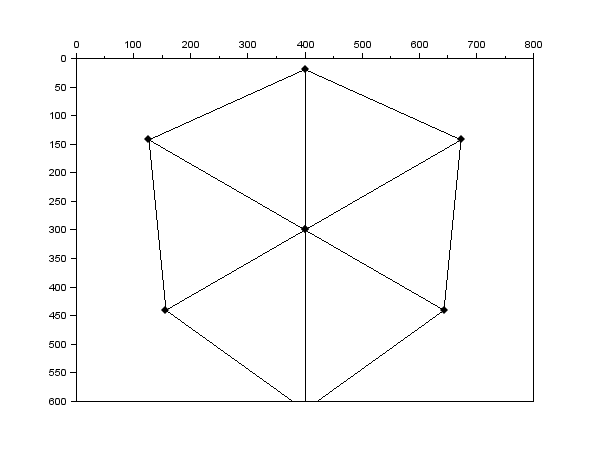
\includegraphics[scale=0.4]{cube_3.png}
\end{figure}

Pour le calcul de la matrice extrinsèque positionnant la caméra d’axe optique selon la diagonale principale du repère, regardant le centre du repère. Centre optique situé à une distance de 5 mètres du centre du repère. Verticale de la caméra dans un plan contenant z; nous devons appliquer tout d’abord une rotation selon l’axe y d’angle -90 degrés, puis une rotation selon l’axe x d’angle arcos(23 ) et enfin une translation selon le vecteur de coordonnées (0,0,5). Ainsi avec ce calcul on obtient la matrice suivante :

\[
   \left (
   \begin{array}{cccc}
      0.7071067811865476 & 0.0 &  -0.7071067811865475     &  0.0\\
-0.40824829046386285     &     0.8164965809277261      &      -0.40824829046386296    & 0.0\\
0.5773502691896258       &      0.5773502691896256      &      0.5773502691896258       & 5.0\\
0.0          &                                 0.0                                         & 0.0                         &             1.0
   \end{array}
   \right )
\]                                1.0


Pour pouvoir appliquer ces transformations , il suffit de multiplier les coordonnées d’un point par ces matrices.

\newpage

\section*{Matrice intrinsèque}
La matrice intrinsèque définit les caractéristiques propres à la caméra,, l'échelle du repère de l’image et sa distance focale. 

\[
   \left (
   \begin{array}{ccc}
      f/Sc & 0 & Oc\\
0 & f/Sl &  Ol\\
0 & 0 & 1
   \end{array}
   \right )
\]

Le f représente la distance focale, Sc et Sl définissent les dimensions du capteur ,  Oc et Ol définissent le centre du repère.

Grâce a cette matrice on pourra observer nos éléments 3D en positionnant la caméra ou on le souhaite dans notre repère.

Pour appliquer cette matrice à notre cube, nous avons multiplier la matrice de notre cube a notre matrice intrinsèque définie ci-dessus, elle même multipliée a une matrice pour la transformer en coordonnées homogènes.

\section*{Projection et affichage des objets}
\begin{figure}[!ht]
\center
	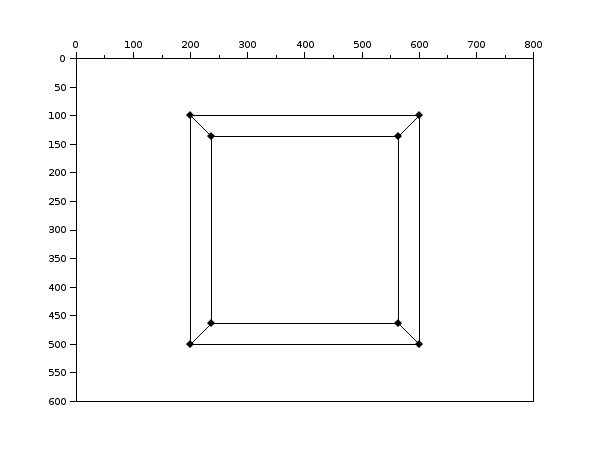
\includegraphics[scale=0.3]{cube_1.png}
	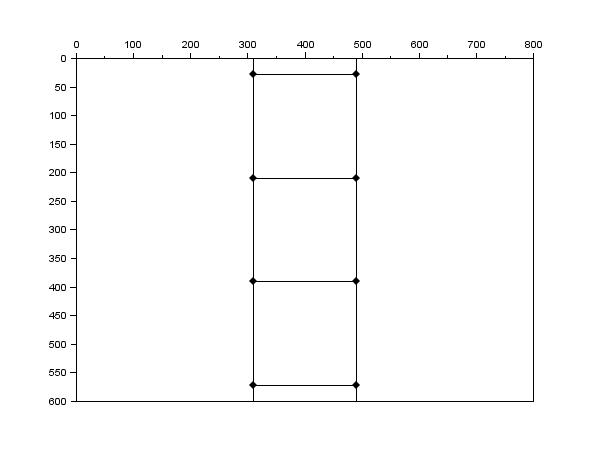
\includegraphics[scale=0.3]{cube_5.png}
	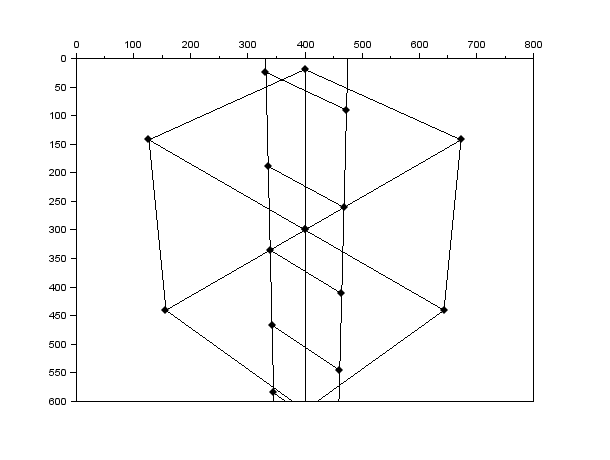
\includegraphics[scale=0.3]{cube_6.png}
\end{figure}

\section*{Conclusion}

Ce TP nous a permis de comprendre comment interpréter des points se trouvant dans un repère 3D dans un repère 2D. Pour cela, nous avons tout d’abord calculer la matrice extrinsèque relative la caméra pour déterminer sa position dans le repère monde. Puis nous avons calculé la matrice intrinsèque afin de régler les paramètres propres à la caméra. Et enfin grâce a ces deux matrices nous avons pu calculer la matrice de projection. Les coordonnées d’un point dans le repère 2D sont calculées en multipliant cette matrice de projection par les coordonnées 3D de ce point.

\end{document}